\begin{figure}[htbp]
  \centering
  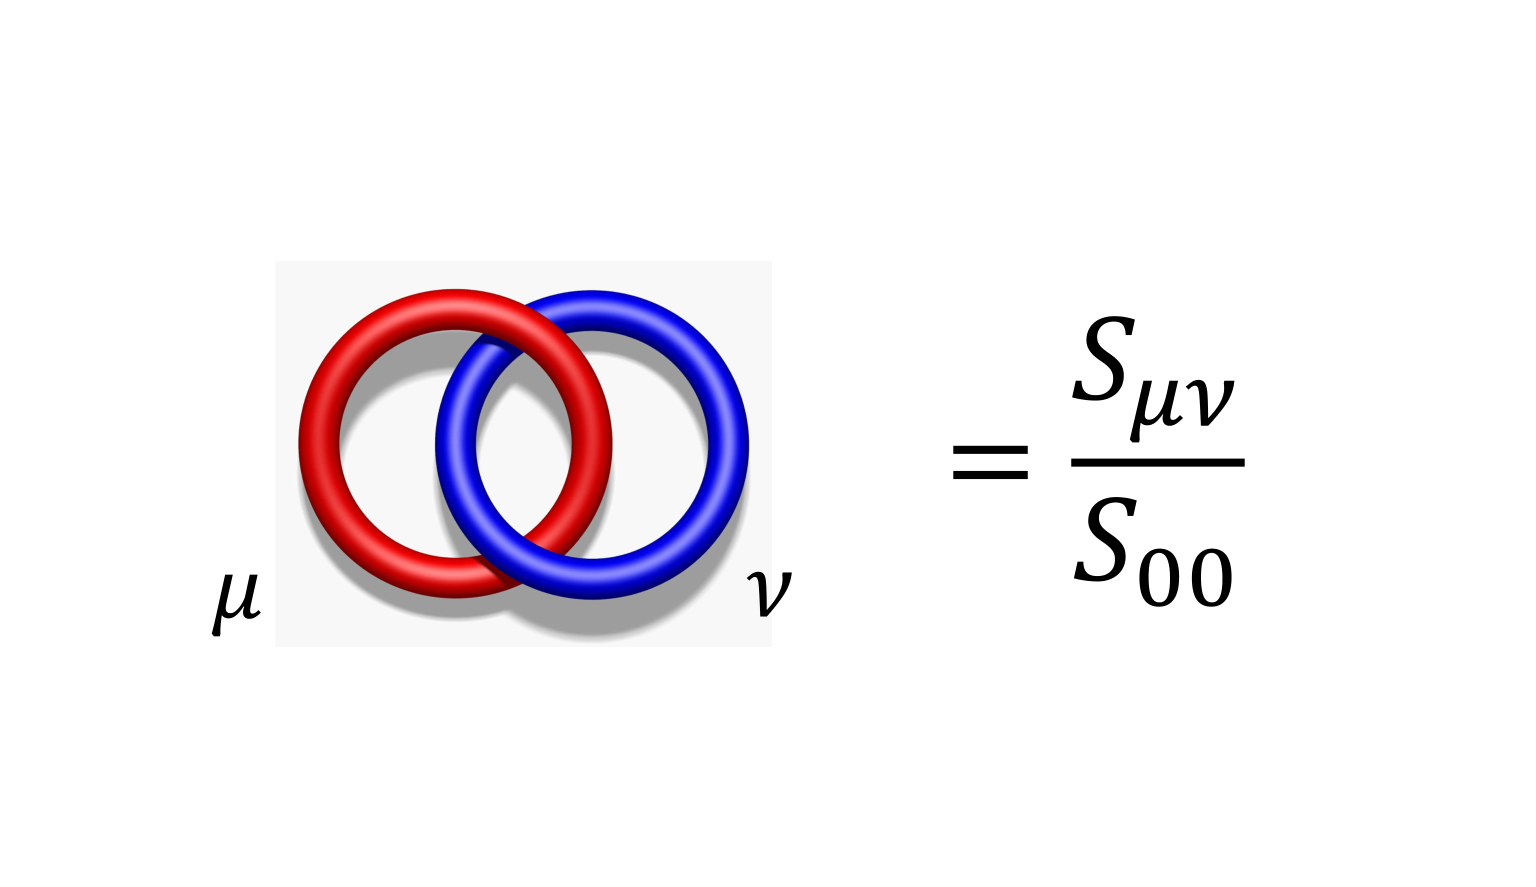
\includegraphics[width=0.60\textwidth]{figures/fig10.png}
  \caption{两条相互链接的圆环，其上分别承载电荷为 $\mu$、$\nu$ 的 Wilson 线缺陷，除此之外不链接任何别的东西；它们等价于一个标量，而这个标量正是模变换 $S$ 在 $\mathcal{H}(T^2)$ 的典范基下的矩阵元 $S_{\mu\nu}$。（原文 Fig.~10，第 72 页）}
  \label{fig:10}
\end{figure}

\begin{enumerate}[start=3]
  \item \underline{与模 $S$ 矩阵的关系。} 特别令人感兴趣的是把关联函数与模 $S$ 矩阵联系起来的一个恒等式。
\end{enumerate}

{\small\itshape ［原文标记：此处已经可以注意到相互链接的圆与模 $S$ 矩阵之间的关系。］}
% [原文待办标记，原文 p.72；其下另有一行星号分隔线，为作者分隔草稿段落所用]

\subsection{与有理共形场论的关系} % 原文: 2.3 Relation To Rational Conformal Field Theory

\subsubsection{\texorpdfstring{$\partial\Sigma$}{∂Σ} 非空时的量子化：边缘态的出现} % 原文: 2.3.1 Quantization When ∂Σ Is Nonempty: Emergence Of Edge States

我们继续考虑 $U(1)$ 能级 $k$ 的 Chern-Simons 理论的量子化。

本节考虑 $M_3=D_2\times\mathbb{R}$，其中 $D_2$ 是一个圆盘。此时出现了边界，因此必须选取边界条件。

一条非常普遍的原则是：\emph{边界条件应当选得使作用量的驻定性成为一个适定的问题。}

换言之，作用量的边界变分应当为零。

{\small\itshape ［原文标记：或许可以用非常一般的辛路径积分来说明，这总归意味着选取一个 Lagrange 子流形。］}
% [原文待办标记，原文 p.72]

在我们的情形中，
\begin{equation}
  \delta\int_{M_3}AdA=\int_{M_3}2\,\delta A\,F+\int_{M_3}d(\delta A\,A)
  \tag{2.299}
  \label{eq:2.299}
\end{equation}
% [Tutor Note: (2.299) 用的是 $\delta(AdA)=\delta A\,dA+A\,d\,\delta A$，第二项分部积分给出恰当形式 $d(\delta A\,A)$，再用 $F=dA$ 把两块合并成 $2\,\delta A\,F$。这里的因子 2 与「无 $\operatorname{tr}$、无 $1/2$」的 $u(1)$ 约定绑定；换到非阿贝尔情形时边界项是 $-\operatorname{tr}(A\,\delta A)$ 型（与 (1.6) 对照），符号与因子都会随之改变，务必统一到 (1.6) 的约定再核对。]

因此我们的边界条件必须使得
\begin{equation}
  \int_{\partial M_3}\delta AA=0
  \tag{2.300}
  \label{eq:2.300}
\end{equation}

最直截了当的做法是在局部强加 $\delta AA|_{\partial M_3}=0$。

在圆盘上取极坐标 $(r,\phi)$，并令 $x^0$ 为时间方向，于是
\begin{equation}
  \delta AA=(\delta A_\phi A_t-\delta A_t A_\phi)\,d\phi\wedge dx^0
  \tag{2.301}
  \label{eq:2.301}
\end{equation}

接下来，我们必须仔细地声明规范变换群是什么。我们把 $A_0$ 视作 Lagrange 乘子，它在 $M_3$ 上强制 $F=0$。于是剩下的规范群只涉及与时间无关的规范变换。

一个有趣的选择是考虑
\begin{equation}
  \mathcal{G}=Map\left(g:D_2\to U(1)\ \middle|\ g|_{\partial D_2}=1\right\}
  \tag{2.302}
  \label{eq:2.302}
\end{equation}
% 原 (2.302) 的定界符本身不配对：左端是圆括号 "("，右端却是花括号 "}"。此处照原样保留（用 \left( ... \right\} 实现），仅加注不加改。
{\small\itshape ［原文标记：这条注记放在这里可能不合适。］}

\textbf{注记}：一般地，若 $X$ 是带边流形，我们考虑群
\begin{equation}
  Map(X\to G)
  \tag{2.303}
  \label{eq:2.303}
\end{equation}
则其中存在由满足 $g|_{\partial X}=1$ 的映射 $g:X\to G$ 组成的子群。在规范场论中，这个子群常被取作描述我们对局部物理之参数化中冗余性的\underline{局部规范变换}群。它是 $Map(X\to G)$ 的正规子群，其商群常被等同于\underline{整体规范变换}群。我们预期态与算符按该群的（可能为射影的）表示变换。

在本情形中可以直截了当地证明 $A_s=ig^{-1}dg=dX$，其中 $X$ 是周期标量场，并且作用量的值只依赖于 $X$ 在边界上的限制：
\begin{equation}
  \int_{D_2\times\mathbb{R}}A_s\partial_0A_s\,dx^0
  =\int_{D_2\times\mathbb{R}}d_s\,(A_s\partial_0X)
  =\int_{\partial D_2\times\mathbb{R}}\partial_\phi X\partial_0X
  \tag{2.304}
  \label{eq:2.304}
\end{equation}
% [Tutor Note: 从 (2.304) 第一式到第二式的关键一步是 $A_s=\partial_sX$（由 $A_s=ig^{-1}\partial_s g=\partial_sX$ 而来），于是 $A_s\partial_0A_s=\tfrac12\partial_0(\partial_sX)^2$；要对 $x^0$ 作一次分部积分（并假定时间方向无边界贡献），才把体积分化为 $\partial D_2\times\mathbb{R}$ 上的边界积分。原文省略了这一步与相应的 $1/2$。此外 $d_s$ 表示只对 $s$ 方向取外微分，别与全微分 $d$ 混用。]

现在让我们回到边界条件，但用 $X$ 来表达它们。我们有
\begin{equation}
  \partial_\phi\delta X\,\partial_tX-\partial_t\delta X\,\partial_\phi X=0
  \tag{2.305}
  \label{eq:2.305}
\end{equation}
若 $X$ 是手征（或反手征）标量场，即可解出
\begin{equation}
  \partial_\phi X\pm\partial_t X=0
  \tag{2.306}
  \label{eq:2.306}
\end{equation}
其中两者取其一，而不可同时取。

{\small\itshape ［原文标记：要提及自对偶场的作用量问题。］}
% [原文待办标记，原文 p.73]

\begin{enumerate}
  \item 如我们所见，在闭三维流形 $M_3$ 上，规范场的 Chern-Simons 不变量 $\frac{1}{4\pi^2}\int_{M_3}AdA$ 的取值只有作为 $\mathbb{R}/\mathbb{Z}$ 的元素才有意义。当 $M_3$ 有非空边界时，情况不同且更为微妙：作用量的值定义了线丛的一个截面。

  {\small\itshape ［原文标记：在这里解释，还是放到后面？？？］}

  \item 反常抵消。我们可以把任意系统与边缘耦合，只要给它配上适当的规范反常，就能得到无反常的系统。
\end{enumerate}

\subsubsection{Wilson 线穿过空间曲面时的量子化} % 原文: 2.3.2 Quantization With Wilson Lines Piercing Spatial Surface

圆盘 $\times\,\mathbb{R}$ 上带 Wilson 线：非平凡和乐。

Gauss 定律中的源。

\subsection{高斯模型：$R^2$ 取有理值的情形} % 原文: 2.4 The Gaussian Model For R^2 Rational

\emph{高斯模型}（Gaussian model）是一个常被用来指代单个无质量标量场（带周期等同）的共形场论的术语。

本节在某种程度上是对共形场论某些简单方面的快速巡览。更详尽的讲述参见：

{\small\itshape ［原文标记：参考文献：Polchinski 第 1 卷；DiFrancesco 等；Fuchs；……？］}
% [原文待办标记，原文 p.74：作者尚未填写的文献指引]

该模型的作用量为
\begin{equation}
  S=K\int dX*dX=K\int d\tau\int_0^{2\pi}d\sigma\left[(\partial_\tau X)^2-(\partial_\sigma X)^2\right]
  \tag{2.307}
  \label{eq:2.307}
\end{equation}
其中 $X$ 无量纲且是周期的（周期可以任意，只要固定下来即可），$K$ 是正常数。

二维的 Green 函数是 $\frac{1}{4\pi}\log|z_1-z_2|^2$，因此
\begin{equation}
  \begin{aligned}
    \langle X(z_1)X(z_2)\rangle&=\frac{1}{2\pi K}\log|z_1-z_2|^2\\
    \langle\partial X(z_1)\partial X(z_2)\rangle&=-\frac{1}{2\pi K}\frac{1}{(z_1-z_2)^2}\,dz_1\wedge dz_2\\
    \langle\bar\partial X(z_1)\bar\partial X(z_2)\rangle&=-\frac{1}{2\pi K}\frac{1}{(\bar z_1-\bar z_2)^2}\,d\bar z_1\wedge d\bar z_2
  \end{aligned}
  \tag{2.308}
  \label{eq:2.308}
\end{equation}

物理学中一种标准的归一化是取 $X\sim X+2\pi$ 以及 $K=\frac{r^2}{4\pi\ell_s^2}$。此时 $X$ 是世界面到半径为 $r$ 的单个圆的映射，而 $\ell_s$ 是弦长。

由运动方程的一般解所定义的高斯场的动量零模与缠绕零模为
\begin{equation}
  X=x_0+\frac{p_L}{\sqrt2}(\tau+\sigma)+\frac{p_R}{\sqrt2}(\tau-\sigma)+X^{\mathrm{osc}}
  \tag{2.309}
  \label{eq:2.309}
\end{equation}
其中我们已取 $\ell_s=1$，$X^{\mathrm{osc}}$ 是非零 Fourier 模的解之和。零模具有这样的性质：向量 $(p_L,p_R)$ 取值于嵌入 $\mathbb{R}^{1,1}$ 的一个偶幺模格中。零模构成的格可写为
\begin{equation}
  \Gamma(r):=\{ne_r+wf_r\,|\,n,w\in\mathbb{Z}\}\subset\mathbb{R}^{1,1}
  \tag{2.310}
  \label{eq:2.310}
\end{equation}
其中
\begin{equation}
  e_r=\frac{1}{\sqrt2}(1/r;1/r),\qquad f_r=\frac{1}{\sqrt2}(r;-r)
  \tag{2.311}
  \label{eq:2.311}
\end{equation}
% [Tutor Note: (2.311) 里的分号 「$;$」 是 Lorentz 型内积下左右手征分量的分隔符，$(v^L;v^R)$ 这种写法与 (2.310) 中 $\mathbb{R}^{1,1}$ 的内积配套。由 $e_r\cdot f_r=1$、$e_r^2=f_r^2=0$ 可验证 $(ne_r+wf_r)^2=2nw$（此处 $p^2=p_L^2-p_R^2$）；若把分号误读成逗号，或误以为 $\{e_r,f_r\}$ 是正交归一对，就会得到 $e_r\cdot f_r=0$ 与 $p^2=n^2+w^2$ 的错误结论。]

注意 $e_r^2=f_r^2=0$、$e_r\cdot f_r=1$，因此 $\Gamma(r)$ 确实是秩 2、符号差 $(1,1)$ 的偶幺模（又称自对偶 Lorentz 型）格 $II^{1,1}$ 的一个嵌入。

该模型具有由流生成的 $u(1)_L\oplus u(1)_R$ 流代数
\begin{equation}
  J_L=\sqrt{\kappa}\sum_{n\in\mathbb{Z}}\alpha_nz^{-n}\frac{dz}{z},
  \qquad
  J_R=\sqrt{\kappa}\sum_{n\in\mathbb{Z}}\tilde\alpha_n\bar z^{-n}\frac{d\bar z}{\bar z}
  \tag{2.312}
  \label{eq:2.312}
\end{equation}
{\small\itshape ［原文标记：这里少了几个恼人的因子 2。］}

我们有
\begin{equation}
  J_L\sim-i\partial X\,\qquad J_R\sim-i\bar\partial X
  \tag{2.313}
  \label{eq:2.313}
\end{equation}
{\small\itshape ［原文标记：恼人的是，在我们的约定下这里有一个非零常数。］}

{\small\itshape ［原文标记：需要对「手征代数」的含义给出更仔细、更形式的讨论。］}
% [原文待办标记，原文 p.75]

它们生成的「手征代数」是由这些场生成的最小的算符乘积代数。忽略左右移动场收缩可能带来的接触项后，我们得到若干个「$u(1)$ 手征代数」的直和。所有这些场都由 $X$ 的（反）全纯导数的多项式得到。我们把它记作 $\mathcal{A}(u(1))$。

{\small\itshape ［原文标记：在此给出手征代数的一般定义；或者推迟，只说这是后面才定义的「手征代数」的一个特例？］}

我们在径向量子化下、于 $SL(2)\times SL(2)$ 不变的真空里计算两点函数：\footnote{这对应于标准归一化
\begin{equation}
  \langle\partial x(z_1)\partial x(z_2)\rangle=-\frac{1}{(z_1-z_2)^2}
  \tag{2.314}
  \label{eq:2.314}
\end{equation}}
\begin{equation}
  \begin{aligned}
    \langle0|J_L(z_1)J_L(z_2)|0\rangle
    &=\kappa\sum_{n=1}^{\infty}n\left(\frac{z_2}{z_1}\right)^{n}\frac{dz_1}{z_1}\otimes\frac{dz_2}{z_2}\\
    &=\frac{\kappa}{(z_1-z_2)^2}\,dz_1\otimes dz_2
  \end{aligned}
  \tag{2.315}
  \label{eq:2.315}
\end{equation}
% [Tutor Note: (2.315) 由级数到闭式用的是一行求和 $\sum_{n\ge1}nx^n=x/(1-x)^2$。取 $x=z_2/z_1$ 得 $\kappa\,z_1z_2/(z_1-z_2)^2$，再乘上 $dz_1/z_1\otimes dz_2/z_2$，两个因子 $z_1z_2$ 恰好相消，才得到最后一行。这也是「必须先设 $|z_1|>|z_2|$ 使级数收敛、再解析延拓」的原因：闭式本身在 $\mathbb{C}\times\mathbb{C}-\mathit{Diag}$ 上单值，但级数不是。]

注意，在径向量子化中我们先在 $|z_1|>|z_2|$ 的区域工作，以使级数收敛；随后由此作解析延拓。对流而言，存在到整个空间 $\mathbb{C}\times\mathbb{C}-\mathit{Diag}$ 的单值解析延拓，没有单值性。

径向量子化中所有关联函数就是这样定义的：理论中的算符要使得关联函数是单值的。

任何手征代数都含有 $T(z)$ 及其全部导数与导数的乘积。注意在此情形
\begin{equation}
  T(z)=-\frac12(\partial x)^2=\frac{1}{2\kappa}:J_L^2:
  \tag{2.316}
  \label{eq:2.316}
\end{equation}
这称为能动张量的 \emph{Sugawara 形式}，它在非阿贝尔情形下将以略微修改的形式成立。

{\small\itshape ［原文标记：$U(1)$ 手征代数的幺正表示（以下为作者以星号框出的草稿段落）：］}
% [原文待办标记，原文 p.76：星号框内的草稿小节，尚未并入正文]

表示：$V_p$，$p\in\mathbb{C}$。幺正表示：$p\in\mathbb{R}$。特征标
\begin{equation}
  \begin{aligned}
    \chi_p&:=\operatorname{Tr}_{V_p}q^{L_0-\frac{c}{24}}e^{2\pi i\xi J_0}\\
    &=\frac{q^{\frac12p^2}e^{2\pi i\xi p}}{\eta}
  \end{aligned}
  \tag{2.317}
  \label{eq:2.317}
\end{equation}

此外，该模型还有顶点算符
\begin{equation}
  V_p(z,\bar z)=c(p):e^{ip_LX(z)}\otimes e^{ip_R\tilde X(\bar z)}:
  \tag{2.318}
  \label{eq:2.318}
\end{equation}
其中动量 $p=(p_L;p_R)$ 被限制在偶幺模格 $\Gamma(r)$ 之中。于是
\begin{equation}
  \begin{aligned}
    p_L&=\frac{1}{\sqrt2}\left(\frac{n}{r}+wr\right)\\
    p_R&=\frac{1}{\sqrt2}\left(\frac{n}{r}-wr\right)
  \end{aligned}
  \tag{2.319}
  \label{eq:2.319}
\end{equation}
其中 $n,w\in\mathbb{Z}$ 分别是动量量子数与缠绕量子数。{\small\itshape ［原文标记：（此处 $c(p)$ 是一个「余闭链算符」——是忽略它，还是解释它？）］} 我们标出了标准的正规序符号。此后我们假定所有取指数形式的顶点算符都带有这一正规序，并在记号中略去不写。

这些场的算符乘积恰好是：
\begin{equation}
  V_{p_1}(1)V_{p_2}(2)=\varepsilon(p_1,p_2)(z_1-z_2)^{p_1^L\cdot p_2^L}(\bar z_1-\bar z_2)^{p_1^R\cdot p_2^R}c(p_1,p_2):e^{i(p_1^LX_L(1)+p_2^LX_L(2))}\otimes e^{i(p_1^RX_R(1)+p_2^RX_R(2))}
  \tag{2.320}
  \label{eq:2.320}
\end{equation}
这里余闭链算符满足 $c(p_1)c(p_2)=\varepsilon(p_1,p_2)c(p_1+p_2)$。它们定义了格 $\Gamma(r)$ 的一个 $\mathbb{Z}_2$ 中心扩张，也就是说，$\varepsilon(p_1,p_2)$ 取值于 $\{\pm1\}$，并且必须满足
\begin{equation}
  \frac{\varepsilon(p_1,p_2)}{\varepsilon(p_2,p_1)}=(-1)^{p_1\cdot p_2}
  \tag{2.321}
  \label{eq:2.321}
\end{equation}
% [Tutor Note: (2.321) 只是 $\varepsilon$ 的相容性条件，它并不能唯一确定 $\varepsilon$；而 (2.320) 中 $\varepsilon(p_1,p_2)$ 与 $c(p_1,p_2)$ 同时出现，正文只说 $c(p_1)c(p_2)=\varepsilon(p_1,p_2)c(p_1+p_2)$，两者的相对归一化（是否把 $\varepsilon$ 吸收进 $c$ 的定义）原文并未固定。计算多顶点关联函数时必须自始至终用同一套约定，否则结果会差出 $\pm1$ 的相位。]

{\small\itshape ［原文标记：解释：］}
\begin{enumerate}
  \item 它是单值的，因为 $p_1\cdot p_2\in\mathbb{Z}$，因为 $\Gamma(r)$ 是整格。
  \item 从而，利用径向量子化与 $SL(2,\mathbb{R})\times SL(2,\mathbb{R})$ 不变的真空：
  \begin{equation}
    \langle\prod_iV_{p_i}(z_i,\bar z_i)\rangle
    =\mathcal{F}_L(z_1,\dots,z_N)\tilde{\mathcal{F}}_R(\bar z_1,\dots,\bar z_N)
    \tag{2.322}
    \label{eq:2.322}
  \end{equation}
  其中
  \begin{equation}
    \mathcal{F}_L(z_1,\dots,z_N)=\prod_{i<j}(z_i-z_j)^{p_i^Lp_j^L}
    \tag{2.323}
    \label{eq:2.323}
  \end{equation}
  被称为该关联函数的\emph{共形块}。
  \item 强调：关联函数是单值的，但共形块具有非平凡的单值性。
\end{enumerate}

对特殊半径，某些 $V_{p_L,p_R}$ 会成为纯全纯算符。这发生在丢番图方程 $p_R=0$ 有解之时。显然这要求
\begin{equation}
  r^2=\frac{m}{w}
  \tag{2.324}
  \label{eq:2.324}
\end{equation}
对某些整数 $m,w$ 成立，因而 $r^2\in\mathbb{Q}$。这些模型称为\emph{有理高斯模型}。它们属于最简单的有理共形场论之列。

{\small\itshape ［原文标记：同样：是否要给出 RCFT 的形式定义？还是推迟？］}

于是，设 $r^2=p/q$ 为既约有理数。则全纯算符由 $m=\ell p$ 与 $w=\ell q$ 得到。它们都是基本全纯顶点算符的各次幂：
\begin{equation}
  V_\pm:=c_\pm e^{i\sqrt{2pq}X}
  \tag{2.325}
  \label{eq:2.325}
\end{equation}
令 $\kappa=pq$。则这些算符具有整数共形维数 $\kappa$，并且绕由 $J_L(z)$ 生成的算符没有单值性，因此可以把它们加到手征代数 $\mathcal{A}(u(1))$ 上，得到更大的手征代数，称为 $u(1)$ 能级 $\kappa$ 手征代数，记作 $\mathcal{A}(u(1))_\kappa$。

$\mathcal{A}(u(1))_\kappa$ 的表示可以在半径 $r^2=p/q$ 处高斯模型顶点算符的全纯部分中找到。它们由「手征顶点算符」生成：
\begin{equation}
  V_n(z)=c\,e^{i\frac{n}{\sqrt{2\kappa}}X(z)}
  \tag{2.326}
  \label{eq:2.326}
\end{equation}

\textbf{警告}：式 \eqref{eq:2.326} 的逻辑地位与 \eqref{eq:2.325} 有重要不同。\eqref{eq:2.326} 中的场本身并不属于高斯模型的谱。左移部分与右移部分必须组合成单值的非全纯场。这与 \eqref{eq:2.325} 相当不同：后者这些场是位于理论的谱中的。

注意 $n\sim n+2\kappa$，而特征标为
\begin{equation}
  \begin{aligned}
    \chi_n(z,\tau)&:=\operatorname{Tr}_{H_n}q^{L_0-\frac{c}{24}}e^{2\pi i\xi J_0}\\
    &=\frac{\sum_{\ell\in\mathbb{Z}}q^{\frac12p_L^2}e^{2\pi i\xi p_L}}{\eta}\\
    &=\frac{\sum_{\ell\in\mathbb{Z}}e^{2\pi i\kappa\tau\left(\ell+\frac{n}{2\kappa}\right)^2+2\pi iz(2\ell\kappa+n)}}{\eta}\\
    &=\frac{\Theta_{n,\kappa}(z,\tau)}{\eta}
  \end{aligned}
  \tag{2.327}
  \label{eq:2.327}
\end{equation}
其中我们定义了 $z=\xi/\sqrt{2\kappa}$，作为在处理模变换与周期性时更方便的归一化。

现在让我们考虑把左移与右移结合起来的 RCFT 的配分函数。在一般半径处我们有
\begin{equation}
  \begin{aligned}
    \operatorname{Tr}_{\mathcal{H}}e^{2\pi i\tau(L_0-\frac{c}{24})+i\xi J_0-2\pi i\bar\tau(\tilde L_0-\frac{\tilde c}{24})-2\pi i\tilde\xi\tilde J_0}
    &=\frac{\sum_{(p_L,p_R)\in\Gamma(r)}q^{\frac12p_L^2}\bar q^{\frac12p_R^2}e^{2\pi i\xi p_L-2\pi i\tilde\xi p_R}}{\eta\bar\eta}\\
    &=\sum_{(p_L,p_R)\in\Gamma(r)}\chi_{p_L}(z,\tau)\overline{\chi_{p_R}(z,\tau)}
  \end{aligned}
  \tag{2.328}
  \label{eq:2.328}
\end{equation}

现在，这个表达式也可以解释为环面上的路径积分：
\begin{equation}
  Z(\tau,\xi;\bar\tau,\bar\xi)
  =e^{-2\frac{(\operatorname{Im}\xi)^2}{\operatorname{Im}\tau}}\operatorname{Tr}_{\mathcal{H}}e^{2\pi i\tau(L_0-\frac{c}{24})+i\xi J_0-2\pi i\bar\tau(\tilde L_0-\frac{\tilde c}{24})-2\pi i\tilde\xi\tilde J_0}
  \tag{2.329}
  \label{eq:2.329}
\end{equation}
其中
\begin{equation}
  Z(\tau,\xi;\bar\tau,\bar\xi)=\int[dX]\,e^{-K\int_\Sigma(\partial X+A^{1,0})\wedge(\bar\partial X+A^{0,1})}
  \tag{2.330}
  \label{eq:2.330}
\end{equation}
并且我们耦合了平坦外场规范场 $A=a_1d\sigma^1+a_2d\sigma^2$，以及
\begin{equation}
  \xi=\mathit{constant}\,\frac{1}{2\pi}(a_2-\bar\tau a_1)
  \tag{2.331}
  \label{eq:2.331}
\end{equation}

该路径积分显然是微分同胚不变的，并且在外场、非动力学 $U(1)$ 规范场 $A$ 的规范变换下是规范不变的。
{\small\itshape ［原文标记：需要核对此式！］}

当一个与度规和/或规范场耦合的路径积分不能适当地规范不变时，我们说存在\emph{反常}。由于我们以对称的方式耦合了左移与右移玻色子，此情形下不可能出现反常。

{\small\itshape ［原文标记：在此给出路径积分计算的细节：］}
\begin{enumerate}
  \item 相关场空间并不连通，且有拓扑上不同的扇区：$X=X_q+X_{sol}$，其中 $X_{sol}=2\pi n^1\sigma^1+2\pi n^2\sigma^2$，$n^1,n^2\in\mathbb{Z}$。
  \item 于是 $Z=Z_q\sum_{n,m}e^{-S_{\mathrm{class}}}$。

  {\small\itshape ［原文标记：给出经典作用量的公式］}

  \item 对 $m$ 作 Poisson 重求和。
  \item 用 $\zeta$ 函数正则化计算 $Z_q$，得到
  \begin{equation}
    Z_q=\frac{1}{\sqrt{\operatorname{Im}\tau}\,|\eta(\tau)|^2}
    \tag{2.332}
    \label{eq:2.332}
  \end{equation}
  \item 评注：对非紧致玻色子我们有
  \begin{equation}
    Z_q=\frac{1}{\sqrt{\operatorname{Im}\tau}\,|\eta(\tau)|^2}
    \tag{2.333}
    \label{eq:2.333}
  \end{equation}
  这可以从 $r\to\infty$ 极限恢复：它来自 Gauss 积分
  \begin{equation}
    \int_{-\infty}^{+\infty}dp\,e^{-\pi\operatorname{Im}\tau\,p^2}
    \tag{2.334}
    \label{eq:2.334}
  \end{equation}
\end{enumerate}
% [Tutor Note: (2.332) 与 (2.333) 的右端逐字相同，这很可能是原稿的笔误，也可能是作者有意强调「两种情形的振荡子行列式部分一致」。(2.333) 的语境是 $r\to\infty$ 的非紧致极限，其额外的动量积分正是 (2.334)；因此 (2.333) 里的 $Z_q$ 应理解为振荡子部分，而非完整的非紧致配分函数。引用时不要由此推断紧致与非紧致玻色子的配分函数相等。]

{\small\itshape ［原文标记：（星号框结束线）］}

现当 $r^2=p/q$ 时，对 Narain 格 $\Gamma(r)$ 的无穷求和会以有趣的方式简化
% 原句在印刷页 p.78 末尾被截断，续见下一片段；此处不补句号，以免造成「句子已完」的错觉。
